\documentclass[aspectratio=169,10pt]{beamer}
\usepackage{fontspec}
\setsansfont{TeX Gyre Heros}
\usepackage{booktabs}
\usepackage{pgfplots}
\usepackage{tikz}
\pgfplotsset{compat=1.18}
\usetikzlibrary{calc,positioning}

\definecolor{Navy}{HTML}{14213D}
\definecolor{Gold}{HTML}{D4A017}
\definecolor{Teal}{HTML}{2A9D8F}
\definecolor{Red}{HTML}{C94C4C}
\definecolor{Gray}{HTML}{6B7280}
\definecolor{LightGray}{HTML}{F5F6F8}
\definecolor{MidGray}{HTML}{D9DEE7}
\definecolor{PaleTeal}{HTML}{E8F5F2}
\definecolor{PaleRed}{HTML}{F9ECEC}
\definecolor{PaleGold}{HTML}{FBF4DF}

\input{presentation_data.tex}
\hypersetup{colorlinks=false,pdfborder={0 0 0},pdfhighlight=/N}
\setbeamertemplate{navigation symbols}{}
\setbeamercolor{normal text}{fg=Navy,bg=white}
\setbeamercolor{frametitle}{fg=Navy,bg=white}
\setbeamerfont{frametitle}{series=\bfseries,size=\fontsize{18.5}{21.5}}
\setbeamertemplate{frametitle}{\vspace{0.08cm}\insertframetitle\par\vspace{0.02cm}\color{Gold}\rule{1.05cm}{1.8pt}\color{Navy}}
\setbeamersize{text margin left=0.66cm,text margin right=0.66cm}
\setbeamertemplate{footline}{\leavevmode\hbox{\begin{beamercolorbox}[wd=.78\paperwidth,ht=0.34cm,dp=0.13cm,leftskip=.66cm]{normal text}\color{Gray}\fontsize{6.2}{7.2}\selectfont Google Review Intelligence \enspace|\enspace Data through \LatestReviewDate\end{beamercolorbox}\begin{beamercolorbox}[wd=.22\paperwidth,ht=0.34cm,dp=0.13cm,rightskip=.66cm plus1fil]{normal text}\color{Gray}\fontsize{6.2}{7.2}\selectfont \insertframenumber/\inserttotalframenumber\end{beamercolorbox}}}
\setbeamertemplate{itemize item}{\color{Gold}\small\raise0.15ex\hbox{\textbullet}}
\setbeamertemplate{enumerate item}{\color{Navy}\bfseries\insertenumlabel.}

\newcommand{\sectiontag}[1]{{\color{Gold}\fontsize{6.8}{8}\selectfont\bfseries\MakeUppercase{#1}}\par\vspace{0.06cm}}
\newcommand{\smallcapslabel}[1]{{\color{Gray}\fontsize{7}{8.2}\selectfont\bfseries\MakeUppercase{#1}}}
\newcommand{\badge}[2]{\begingroup\setlength{\fboxsep}{0.07cm}\colorbox{#1}{\color{Navy}\fontsize{6.1}{7.2}\selectfont\bfseries #2}\endgroup}
\newcommand{\sourceReview}{\badge{PaleTeal}{CUSTOMER/DATA EVIDENCE}}
\newcommand{\sourceInternal}{\badge{PaleGold}{INTERNAL OBSERVATION}}
\newcommand{\sourceExperiment}{\badge{PaleRed}{PROPOSED EXPERIMENT}}
\newcommand{\sourceData}{\badge{LightGray}{DATA REQUIRED}}
\newcommand{\pillbutton}[3]{\begingroup\setlength{\fboxsep}{0.10cm}\hyperlink{#1}{\colorbox{#3}{\color{white}\fontsize{6.8}{8}\selectfont\bfseries #2\ $\rightarrow$}}\endgroup}
\newcommand{\goldbutton}[2]{\pillbutton{#1}{#2}{Gold}}
\newcommand{\tealbutton}[2]{\pillbutton{#1}{#2}{Teal}}
\newcommand{\redbutton}[2]{\pillbutton{#1}{#2}{Red}}
\newcommand{\backbutton}[2]{\begingroup\setlength{\fboxsep}{0.10cm}\hyperlink{#1}{\colorbox{Navy}{\color{white}\fontsize{6.8}{8}\selectfont\bfseries $\leftarrow$\ #2}}\endgroup}
\newcommand{\quotebox}[3]{\begingroup\setlength{\fboxsep}{0.12cm}\colorbox{#1}{\parbox{\dimexpr\linewidth-0.24cm\relax}{\raggedright{\fontsize{7.7}{9.2}\selectfont\itshape ``#2''}\par\vspace{0.04cm}{\color{Gray}\fontsize{5.9}{7}\selectfont #3}}}\endgroup}
\newcommand{\quoteneg}[2]{\quotebox{PaleRed}{#1}{#2}}
\newcommand{\quotepos}[2]{\quotebox{PaleTeal}{#1}{#2}}
\newcommand{\quotegray}[2]{\quotebox{LightGray}{#1}{#2}}
\newcommand{\kpicard}[4]{\colorbox{#1}{\parbox[c][1.18cm][c]{0.92\linewidth}{\centering\smallcapslabel{#2}\par\vspace{0.04cm}{\color{#4}\fontsize{20}{22}\selectfont\bfseries #3}}}}
\newcommand{\countsentimentbar}[3]{\begin{tikzpicture}[x=0.058cm,y=1cm]\pgfmathsetmacro{\PosEnd}{#1/(#1+#2+#3)*100}\pgfmathsetmacro{\NeuEnd}{(#1+#2)/(#1+#2+#3)*100}\fill[Teal,rounded corners=1.2pt] (0,0) rectangle (\PosEnd,0.38);\fill[Gray!35] (\PosEnd,0) rectangle (\NeuEnd,0.38);\fill[Red] (\NeuEnd,0) rectangle (100,0.38);\end{tikzpicture}}
\newcommand{\implication}[1]{\colorbox{Navy}{\parbox{0.965\linewidth}{\color{white}\fontsize{7.6}{9}\selectfont\textbf{Management implication:} #1}}}
\newcommand{\evidenceitem}[3]{{\fontsize{7.7}{9.2}\selectfont\textbf{#1}\hfill #2\quad #3}\par\vspace{0.07cm}}
\newcommand{\appendixhead}[1]{\sectiontag{Evidence Appendix #1}\vspace{0.05cm}}
\newcommand{\casecard}[6]{\begingroup\setlength{\fboxsep}{0.09cm}\colorbox{LightGray}{\parbox[c][2.18cm][t]{0.975\linewidth}{\vspace{0.05cm}{\color{Navy}\fontsize{7}{8.1}\selectfont\bfseries #1\quad #2}\par\vspace{0.02cm}{\fontsize{6.35}{7.45}\selectfont #3}\par{\color{Gray}\fontsize{6.05}{7.15}\selectfont #4}\par{\fontsize{6.25}{7.35}\selectfont\itshape #5}\par\vfill\hfill #6}}\endgroup\par\vspace{0.08cm}}
\newcommand{\opcasecard}[6]{\begingroup\setlength{\fboxsep}{0.09cm}\colorbox{LightGray}{\parbox[c][2.49cm][t]{0.975\linewidth}{\vspace{0.05cm}{\color{Navy}\fontsize{7}{8.1}\selectfont\bfseries #1\quad #2}\par\vspace{0.02cm}{\fontsize{6.35}{7.45}\selectfont #3}\par{\color{Gray}\fontsize{6.05}{7.15}\selectfont #4}\par{\fontsize{6.25}{7.35}\selectfont\itshape #5}\par\vfill\hfill #6}}\endgroup\par\vspace{0.08cm}}
\newcommand{\dishcard}[4]{\begingroup\setlength{\fboxsep}{0.09cm}\colorbox{PaleTeal}{\parbox[c][1.54cm][t]{0.975\linewidth}{\vspace{0.04cm}{\color{Navy}\fontsize{7.2}{8.3}\selectfont\bfseries #1}\par{\fontsize{6.2}{7.3}\selectfont #2}\par{\fontsize{6.1}{7.2}\selectfont\itshape ``#3''}\hfill #4}}\endgroup\par\vspace{0.06cm}}
\newcommand{\chapterdivider}[7]{\begin{frame}[plain]\hypertarget{#6}{}\begin{tikzpicture}[remember picture,overlay]\fill[Navy] (current page.south west) rectangle (current page.north east);\fill[#7] (current page.south west) rectangle ([xshift=0.18cm]current page.north west);\end{tikzpicture}\vfill{\color{#7}\fontsize{10}{12}\selectfont\bfseries CHAPTER #1}\par\vspace{0.14cm}{\color{white}\fontsize{28}{32}\selectfont\bfseries #2}\par\vspace{0.34cm}\begin{columns}[T,onlytextwidth]\column{0.31\textwidth}{\color{white!55}\fontsize{6.5}{7.5}\selectfont\bfseries WHAT IT PROVES}\par\vspace{0.05cm}{\color{white}\fontsize{8}{9.5}\selectfont #3}\column{0.31\textwidth}{\color{white!55}\fontsize{6.5}{7.5}\selectfont\bfseries WHY IT MATTERS}\par\vspace{0.05cm}{\color{white}\fontsize{8}{9.5}\selectfont #4}\column{0.31\textwidth}{\color{white!55}\fontsize{6.5}{7.5}\selectfont\bfseries ACTION SUPPORTED}\par\vspace{0.05cm}{\color{white}\fontsize{8}{9.5}\selectfont #5}\end{columns}\vfill\goldbutton{#6-content}{Open chapter}\end{frame}}

\begin{document}

\begin{frame}[plain]
  \hypertarget{m-cover}{}\begin{tikzpicture}[remember picture,overlay]\fill[Navy] (current page.south west) rectangle (current page.north east);\fill[Gold] (current page.south west) rectangle ([xshift=0.20cm]current page.north west);\fill[Gold,opacity=.17] ([xshift=-4.3cm,yshift=-1.0cm]current page.north east) circle (3.1cm);\fill[Teal,opacity=.14] ([xshift=-1.1cm,yshift=1.0cm]current page.south east) circle (2.15cm);\end{tikzpicture}
  \vspace{0.85cm}{\color{Gold}\fontsize{9.5}{11.5}\selectfont\bfseries MANAGEMENT REVIEW INTELLIGENCE}\par\vspace{0.38cm}{\color{white}\fontsize{34}{38}\selectfont\bfseries Al Assiel Restaurant\\[-0.02cm]\& Shisha}\par\vspace{0.25cm}{\color{white!82}\fontsize{14}{18}\selectfont Executive story, operational evidence and action ownership}\par\vfill{\color{white}\fontsize{10}{12}\selectfont Bonn, Germany}\par\vspace{0.08cm}{\color{white!68}\fontsize{8.4}{10}\selectfont \TotalReviews\ Google reviews | \WrittenReviews\ written reviews | Data through \LatestReviewDate}\vspace{0.44cm}
\end{frame}

\begin{frame}{Presentation Roadmap}
  \hypertarget{m-roadmap}{}\sectiontag{How to use this deck}
  \begin{columns}[T,onlytextwidth]
    \column{0.48\textwidth}{\fontsize{7.2}{8.6}\selectfont\textbf{1 Executive Overview}\quad Main story and priority\par\textbf{2 Last-Month Performance}\quad Latest vs previous 30d\par\textbf{3 Performance Trends}\quad Monthly and 90d context\par\textbf{4 Review Flow \& Response}\quad Cadence and follow-up\par\textbf{5 Bad Reviews}\quad Patterns and 30 operational cases\par\textbf{6 Service}\quad Repeated weakness evidence\par\textbf{7 Kitchen / Food / Taste}\quad Strength plus recent checks\par\textbf{8 Bar \& Drinks}\quad Attention and experience signals}
    \column{0.48\textwidth}{\fontsize{7.2}{8.6}\selectfont\textbf{9 Buffet}\quad Sentiment and monitoring needs\par\textbf{10 Menu \& Ordering}\quad Review limits and POS needs\par\textbf{11 Dishes Mentioned}\quad All observed items\par\textbf{12 Management Observations}\quad Provenance-separated inputs\par\textbf{13 Action Plan}\quad Immediate vs evidence-dependent work\par\textbf{14 Delegation}\quad Four accountable workstreams\par\textbf{15 KPI Tracking}\quad Weekly control dashboard\par\textbf{16 Evidence Appendix}\quad Case registers, links and checklists}
  \end{columns}
  \vfill\goldbutton{m-ch1}{Start Chapter 1}\quad\tealbutton{m-ch16}{Open Evidence Appendix}
\end{frame}

\chapterdivider{1}{Executive Overview}{The lifetime reputation is strong, but recent experience and follow-up are weaker.}{Management should protect the brand while acting on current operating signals.}{Set the management priority and open the evidence only where needed.}{m-ch1}{Gold}

\begin{frame}{Strong reputation; recent performance still needs attention}
  \hypertarget{m-ch1-content}{}\hypertarget{m-exec}{}\sectiontag{Chapter 1 - Executive Overview}
  \begin{columns}[T,onlytextwidth]\column{0.235\textwidth}\kpicard{PaleGold}{Google rating}{\GoogleRating}{Gold}\column{0.235\textwidth}\kpicard{LightGray}{Total reviews}{\TotalReviews}{Navy}\column{0.235\textwidth}\kpicard{PaleTeal}{Historical avg.}{\HistoricalAverage}{Teal}\column{0.235\textwidth}\kpicard{PaleRed}{Recent 90d avg.}{\RecentNinetyAverage}{Red}\end{columns}
  \vspace{0.25cm}\begin{columns}[T,onlytextwidth]\column{0.48\textwidth}\smallcapslabel{What remains strong}\par\vspace{0.08cm}{\fontsize{9}{10.8}\selectfont Collected average \CollectedAverage; \PositiveRatingPct\% of ratings are 4-5 stars. Food, Taste and friendliness remain visible strengths.}\column{0.48\textwidth}\smallcapslabel{What needs control}\par\vspace{0.08cm}{\fontsize{9}{10.8}\selectfont Recent 90d: \RecentNinetyAverage\ across \RecentNinetyReviews\ reviews, \RecentNegativePct\% negative vs \HistoricalNegativePct\% historically. Owner response remains weak.}\end{columns}
  \vfill\implication{Protect strengths, restore the recent experience, and close the response-loop gap.}\par\vspace{0.08cm}\goldbutton{a-trend}{View trend evidence}\quad\redbutton{a-bad-register}{View 30 bad-review cases}
\end{frame}

\chapterdivider{2}{Last-Month Performance}{The latest 30d improved versus the prior 30d, but four low-score cases remain.}{Averages alone can hide open cases and low-evidence emerging topics.}{Review all 14 recent cases and compare them with the six prior cases.}{m-ch2}{Teal}

\begin{frame}{Latest 30 days improved, with four low-score cases still open}
  \hypertarget{m-ch2-content}{}\hypertarget{m-lastmonth}{}\sectiontag{Chapter 2 - Last-Month Performance}
  {\color{Gray}\fontsize{6.5}{7.7}\selectfont Latest 30 days: \RecentThirtyStart\ to \LatestReviewDate. Previous 30 days: \PreviousThirtyStart\ to \RecentThirtyStart.}
  \vspace{0.10cm}\begin{columns}[T,onlytextwidth]\column{0.47\textwidth}\smallcapslabel{Latest 30 days}\par\vspace{0.07cm}\begin{columns}[T,onlytextwidth]\column{0.48\textwidth}\kpicard{PaleTeal}{Average}{\RecentThirtyAverage}{Teal}\column{0.48\textwidth}\kpicard{LightGray}{Reviews}{\RecentThirtyReviews}{Navy}\end{columns}\vspace{0.10cm}{\fontsize{8}{9.5}\selectfont \RecentThirtyWritten\ written | \RecentThirtyPerWeek/week | \RecentThirtyNegativePct\% negative | \RecentThirtyLowScores\ low-score | \OwnerRecentThirtyRate\% response}\column{0.47\textwidth}\smallcapslabel{Previous 30 days}\par\vspace{0.07cm}\begin{columns}[T,onlytextwidth]\column{0.48\textwidth}\kpicard{LightGray}{Average}{\PreviousThirtyAverage}{Navy}\column{0.48\textwidth}\kpicard{LightGray}{Reviews}{\PreviousThirtyReviews}{Navy}\end{columns}\vspace{0.10cm}{\fontsize{8}{9.5}\selectfont \PreviousThirtyWritten\ written | \PreviousThirtyPerWeek/week | \PreviousThirtyNegativePct\% negative | \PreviousThirtyLowScores\ low-score | \OwnerPreviousThirtyRate\% response}\end{columns}
  \vspace{0.16cm}\colorbox{PaleTeal}{\parbox{0.95\linewidth}{\centering\fontsize{8.5}{10}\selectfont Average +\RecentThirtyDelta\ stars; negative share -\RecentThirtyNegativeDeltaAbs\ pp; volume \PreviousThirtyReviews\ $\rightarrow$ \RecentThirtyReviews. Improvement does not close the four low-score cases.}}
  \vfill\goldbutton{a-latest-summary}{View detailed comparison}\quad\redbutton{a-latest-register}{View all 14 recent cases}\quad\tealbutton{a-previous-register}{View six prior cases}
\end{frame}

\begin{frame}{The 30-day improvement contains mixed and low-evidence signals}
  \hypertarget{m-lastmonth-detail}{}\sectiontag{Chapter 2 - Topic-level comparison}
  \begin{columns}[T,onlytextwidth]\column{0.31\textwidth}\colorbox{PaleTeal}{\parbox[c][4.15cm][t]{0.92\linewidth}{\vspace{0.13cm}\smallcapslabel{Improved}\par\vspace{0.12cm}{\fontsize{8.4}{10}\selectfont Taste and Service each had \textbf{\RecentThirtyTastePositive\ positive reviews}. Overall average improved and review cadence increased. Evidence labels are based on supporting sentiment reviews.}}}\column{0.31\textwidth}\colorbox{PaleRed}{\parbox[c][4.15cm][t]{0.92\linewidth}{\vspace{0.13cm}\smallcapslabel{Needs review}\par\vspace{0.12cm}{\fontsize{8.4}{10}\selectfont Food had \textbf{\RecentThirtyFoodNegative\ negative reviews} (\RecentThirtyFoodNegativeEvidence\ evidence). Four low-score reviews arrived; none received an owner response.}}}\column{0.31\textwidth}\colorbox{PaleGold}{\parbox[c][4.15cm][t]{0.92\linewidth}{\vspace{0.13cm}\smallcapslabel{Still unclear}\par\vspace{0.12cm}{\fontsize{8.4}{10}\selectfont Taste, Service, Menu/Tablet, communication and parking each have only one negative recent review. Drinks has two neutral mentions. Investigate; do not overstate.}}}\end{columns}
  \vfill\goldbutton{a-latest-summary}{View counts and chart}\quad\redbutton{a-latest-register}{Open case register}
\end{frame}

\chapterdivider{3}{Performance Trends}{Recent 90d performance sits below the historical pattern across rating and negative share.}{Monthly edges are partial and the lifetime score moves slowly.}{Use rolling 30d/90d control and inspect volume plus low-score counts.}{m-ch3}{Gold}

\begin{frame}{Monthly rating shows a recent gap; edge months are partial}
  \hypertarget{m-ch3-content}{}\hypertarget{m-trend}{}\sectiontag{Chapter 3 - Monthly Average Rating}
  \begin{columns}[T,onlytextwidth]\column{0.69\textwidth}\begin{tikzpicture}\begin{axis}[width=10.0cm,height=4.7cm,xmin=-0.5,xmax=21.5,ymin=2.4,ymax=5.15,axis line style={Gray!45},tick style={Gray!45},monthly axis ticks,x tick label style={font=\fontsize{6}{7}\selectfont},ytick={3,4,5},yticklabel style={font=\scriptsize},grid=major,grid style={LightGray},ylabel={Average rating},ylabel style={font=\scriptsize}]\addplot[Navy,very thick,mark=*,mark size=1.6pt] table[x=index,y=average,col sep=comma]{assets/monthly_trend.csv};\addplot[Gold,only marks,mark=*,mark size=4pt] table[x=index,y=average,col sep=comma]{assets/monthly_partial.csv};\addplot[Gray,dashed,thick,domain=-0.5:21.5] {\HistoricalAverage};\end{axis}\end{tikzpicture}\column{0.27\textwidth}\smallcapslabel{Recent 90d}\par{\color{Red}\fontsize{21}{23}\selectfont\bfseries \RecentNinetyAverage}\par{\color{Gray}\scriptsize \RecentNinetyReviews\ reviews | \RecentNegativePct\% negative}\par\vspace{0.14cm}\smallcapslabel{Historical}\par{\fontsize{17}{19}\selectfont\bfseries \HistoricalAverage}\par{\color{Gray}\scriptsize \HistoricalReviews\ reviews | \HistoricalNegativePct\% negative}\par\vspace{0.16cm}{\fontsize{7.2}{8.6}\selectfont Gold points mark partial Dec 2024 and Sep 2026. Do not treat them as full-month volumes.}\end{columns}
  \vfill{\color{Gray}\fontsize{6.5}{7.7}\selectfont Historical: \EarliestReviewDate\ to \RecentNinetyStart. Recent 90d: \RecentNinetyStart\ to \LatestReviewDate.}\par\vspace{0.07cm}\goldbutton{a-trend}{View trend evidence}
\end{frame}

\begin{frame}{Review volume and low-score volume must be read together}
  \hypertarget{m-trend-volume}{}\sectiontag{Chapter 3 - Volume and Recent-vs-Historical Comparison}
  \begin{columns}[T,onlytextwidth]\column{0.48\textwidth}\begin{tikzpicture}\begin{axis}[ybar,bar width=5pt,width=7.0cm,height=4.35cm,xmin=-0.6,xmax=21.6,ymin=0,ymax=24,monthly axis ticks,x tick label style={font=\fontsize{5.5}{6.5}\selectfont},ytick={0,5,10,15,20},yticklabel style={font=\scriptsize},grid=major,grid style={LightGray},ylabel={Monthly reviews},ylabel style={font=\scriptsize}]\addplot[fill=Teal,draw=Teal] table[x=index,y=reviews,col sep=comma]{assets/review_volume.csv};\end{axis}\end{tikzpicture}\par{\color{Gray}\fontsize{6.2}{7.3}\selectfont Monthly volume; Dec 2024 and Sep 2026 are partial.}\column{0.48\textwidth}\begin{tikzpicture}\begin{axis}[ybar,bar width=13pt,width=7.0cm,height=4.35cm,symbolic x coords={Historical,Previous90,Recent90},xtick=data,xticklabels={Historical,Previous 90d,Recent 90d},x tick label style={font=\fontsize{5.8}{6.8}\selectfont},ytick={0,10,20,30,40},yticklabel style={font=\scriptsize},grid=major,grid style={LightGray},ylabel={Negative share (\%)},ylabel style={font=\scriptsize}]\addplot[fill=Red,draw=Red] table[x=period,y=negative_pct,col sep=comma]{assets/period_rating_comparison.csv};\end{axis}\end{tikzpicture}\par{\color{Gray}\fontsize{6.2}{7.3}\selectfont Recent 90d negative share is materially above history; period count is \RecentNinetyReviews.}\end{columns}
  \vfill\goldbutton{a-trend}{View monthly tables and structured trends}
\end{frame}

\chapterdivider{4}{Review Flow \& Owner Response}{Reviews arrive frequently enough to detect change, but recent owner response is inactive.}{Unanswered feedback leaves recovery and learning opportunities open.}{Assign a response owner, deadline and closure process.}{m-ch4}{Teal}

\begin{frame}{Feedback arrives every two days; the response loop is inactive}
  \hypertarget{m-ch4-content}{}\hypertarget{m-owner}{}\sectiontag{Chapter 4 - Review Flow \& Owner Response}
  \begin{columns}[T,onlytextwidth]\column{0.57\textwidth}\begin{tikzpicture}\begin{axis}[ybar,bar width=17pt,width=8.2cm,height=4.55cm,ymin=0,ymax=16,symbolic x coords={0,1,2},xtick=data,xticklabels={Historical,Previous 90d,Recent 90d},x tick label style={font=\fontsize{6.2}{7.2}\selectfont},ytick={0,5,10,15},yticklabel style={font=\scriptsize},legend style={font=\fontsize{5.8}{6.8}\selectfont,at={(0.5,1.02)},anchor=south,legend columns=2,draw=none},grid=major,grid style={LightGray}]\addplot[fill=Gold,draw=Gold] table[x=index,y=rate,col sep=comma]{assets/owner_response_periods.csv};\addplot[fill=Red,draw=Red] table[x=index,y=low_score_rate,col sep=comma]{assets/owner_response_periods.csv};\legend{All reviews,Low-score}\end{axis}\end{tikzpicture}\column{0.39\textwidth}\begin{columns}[T,onlytextwidth]\column{0.48\textwidth}\kpicard{PaleGold}{Overall response}{\OwnerOverallRate\%}{Gold}\column{0.48\textwidth}\kpicard{PaleRed}{Recent 30d}{\OwnerRecentThirtyRate\%}{Red}\end{columns}\vspace{0.12cm}\begin{columns}[T,onlytextwidth]\column{0.48\textwidth}\kpicard{PaleRed}{Low-score}{\LowScoreResponseRate\%}{Red}\column{0.48\textwidth}\kpicard{PaleRed}{Unanswered}{\LowScoreUnanswered/\LowScoreReviews}{Red}\end{columns}\vspace{0.12cm}{\fontsize{7.4}{8.8}\selectfont Latest 30d cadence: \RecentThirtyPerWeek/week; one review every \RecentThirtyGap\ days. Median delay among answered reviews: \OwnerMedianDelay\ days.}\end{columns}
  \vfill{\color{Gray}\fontsize{6.4}{7.6}\selectfont Periods: historical \EarliestReviewDate-\RecentNinetyStart; recent 90d \RecentNinetyStart-\LatestReviewDate.}\par\vspace{0.07cm}\goldbutton{a-owner}{View response evidence}\quad\redbutton{a-response-process}{View closure process}
\end{frame}

\chapterdivider{5}{Bad Reviews / Low-Score Cases}{Thirty 1-2 star reviews define a finite operational workload with repeated Service, Food and Value issues.}{Twenty-nine are unanswered; vague summaries are not enough for closure.}{Assign every case, examine patterns, respond and document internal checks.}{m-ch5}{Red}

\begin{frame}{Thirty bad reviews define the follow-up workload}
  \hypertarget{m-ch5-content}{}\hypertarget{m-badscale}{}\sectiontag{Chapter 5 - Bad-Review Scale}
  \begin{columns}[T,onlytextwidth]\column{0.42\textwidth}\begin{columns}[T,onlytextwidth]\column{0.48\textwidth}\kpicard{PaleRed}{1-star}{\OneStarReviews}{Red}\par{\centering\color{Gray}\scriptsize \OneStarWritten\ written}\column{0.48\textwidth}\kpicard{PaleGold}{2-star}{\TwoStarReviews}{Gold}\par{\centering\color{Gray}\scriptsize \TwoStarWritten\ written}\end{columns}\vspace{0.20cm}{\fontsize{23}{25}\selectfont\bfseries \LowScoreReviews}\quad{\color{Red}\large \LowScoreShare\% of all reviews}\par{\color{Gray}\fontsize{7.2}{8.6}\selectfont \LowScoreWritten\ written; \LowScoreUnanswered\ unanswered. Latest 30d: \RecentThirtyLowScores. Recent 90d: \RecentLowScores.}\column{0.54\textwidth}\begin{tikzpicture}\begin{axis}[ybar,bar width=6pt,width=7.8cm,height=4.45cm,xmin=-0.6,xmax=21.6,ymin=0,ymax=6,monthly axis ticks,x tick label style={font=\fontsize{5.8}{6.8}\selectfont},ytick={0,1,2,3,4,5},yticklabel style={font=\scriptsize},ylabel={1-2 star reviews},ylabel style={font=\scriptsize},grid=major,grid style={LightGray}]\addplot[fill=Red,draw=Red] table[x=index,y=low_scores,col sep=comma]{assets/monthly_trend.csv};\end{axis}\end{tikzpicture}\par{\color{Gray}\fontsize{6.2}{7.3}\selectfont Monthly low-score volume; edge months are partial.}\end{columns}
  \vfill\redbutton{a-bad-register}{Open all 30 cases}\quad\goldbutton{a-bad-patterns}{View pattern analysis}
\end{frame}

\begin{frame}{Repeated bad-review issues and co-occurrences guide investigation}
  \hypertarget{m-badpatterns}{}\sectiontag{Chapter 5 - Pattern Map}
  \begin{columns}[T,onlytextwidth]\column{0.48\textwidth}\smallcapslabel{Repeated negative areas}\par\vspace{0.08cm}\evidenceitem{Service}{\LowServiceCount\ | \LowServicePct\%}{\badge{PaleRed}{\LowServiceEvidence}}\evidenceitem{Food}{\LowFoodCount\ | \LowFoodPct\%}{\badge{PaleGold}{\LowFoodEvidence}}\evidenceitem{Price \& Value}{\LowPriceCount\ | \LowPricePct\%}{\badge{PaleGold}{\LowPriceEvidence}}\evidenceitem{Taste}{\LowTasteCount\ | \LowTastePct\%}{\badge{LightGray}{\LowTasteEvidence}}\evidenceitem{Menu/Tablet}{\LowMenuCount\ | low volume}{\badge{LightGray}{LOW}}\column{0.48\textwidth}\smallcapslabel{Co-occurrence chart}\par\vspace{0.06cm}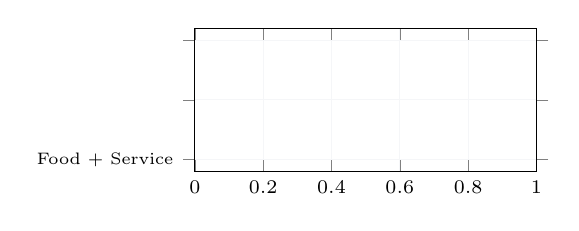
\begin{tikzpicture}\begin{axis}[xbar,width=5.92cm,height=3.4cm,xmin=0,xmax=4,symbolic y coords={Price+Service,Food+Service},ytick=data,yticklabels={Price/Value + Service,Food + Service},y tick label style={font=\fontsize{6.1}{7.1}\selectfont},xtick={0,1,2,3,4},xticklabel style={font=\scriptsize},grid=major,grid style={LightGray}]\addplot[fill=Red,draw=Red] coordinates {(\LowPairTwoCount,Price+Service) (\LowPairOneCount,Food+Service)};\end{axis}\end{tikzpicture}\par{\fontsize{7}{8.4}\selectfont All other pairs occur once. Co-occurrence directs internal checks; it does not prove root cause. Day/time and shift data are unavailable.}\end{columns}
  \vfill\goldbutton{a-bad-patterns}{View full patterns}\quad\redbutton{a-bad-cooccurrence}{View recent shift}
\end{frame}

\begin{frame}{Treat every bad review as an operational case, not a quote}
  \hypertarget{m-badcases}{}\sectiontag{Chapter 5 - Operational Case Design}
  \begin{columns}[T,onlytextwidth]\column{0.31\textwidth}\colorbox{PaleRed}{\parbox[c][3.75cm][t]{0.92\linewidth}{\vspace{0.14cm}\smallcapslabel{Case intake}\par\vspace{0.10cm}{\fontsize{8.2}{9.8}\selectfont Anonymous case ID, rating/date, positive/negative topics, item/buffet/drinks/menu flags, written/no-text and public original-review link.}}}\column{0.31\textwidth}\colorbox{PaleGold}{\parbox[c][3.75cm][t]{0.92\linewidth}{\vspace{0.14cm}\smallcapslabel{Ownership}\par\vspace{0.10cm}{\fontsize{8.2}{9.8}\selectfont Proposed workstream owner, 48-hour public-response target, issue-specific internal check and response date when available.}}}\column{0.31\textwidth}\colorbox{PaleTeal}{\parbox[c][3.75cm][t]{0.92\linewidth}{\vspace{0.14cm}\smallcapslabel{Closure}\par\vspace{0.10cm}{\fontsize{8.2}{9.8}\selectfont Keep the case open until the internal check and action are documented. Current internal-resolution fields are unavailable.}}}\end{columns}
  \vfill\redbutton{a-bad-register}{View 30-case register}\quad\goldbutton{a-response-process}{View response checklist}
\end{frame}

\chapterdivider{6}{Service}{Service is mostly positive, yet it is the clearest repeated weakness in low-score reviews.}{Repeated waiting, responsiveness and communication failures can outweigh many positive mentions.}{Investigate all negative cases by journey stage and future shift/time fields.}{m-ch6}{Teal}

\begin{frame}{Service is positive overall and still the clearest recurring weakness}
  \hypertarget{m-ch6-content}{}\hypertarget{m-service}{}\sectiontag{Chapter 6 - Service}
  \begin{columns}[T,onlytextwidth]\column{0.48\textwidth}\smallcapslabel{Historical}\par\vspace{0.07cm}\countsentimentbar{\ServicePeriodHistoricalPositive}{\ServicePeriodHistoricalNeutral}{\ServicePeriodHistoricalNegative}\par{\color{Gray}\fontsize{6.7}{8}\selectfont \ServicePeriodHistoricalMentions\ mentions | \ServicePeriodHistoricalNegative\ negative | \ServicePeriodHistoricalNegativeEvidence\ weakness evidence}\par\vspace{0.15cm}\smallcapslabel{Recent 90d}\par\vspace{0.07cm}\countsentimentbar{\ServicePeriodRecentPositive}{\ServicePeriodRecentNeutral}{\ServicePeriodRecentNegative}\par{\color{Gray}\fontsize{6.7}{8}\selectfont \ServicePeriodRecentMentions\ mentions | \ServicePeriodRecentNegative\ negative | \ServicePeriodRecentNegativeEvidence\ weakness evidence}\par\vspace{0.15cm}{\fontsize{7.8}{9.3}\selectfont Latest 30d: \RecentThirtyServiceMentions\ mentions; \RecentThirtyServiceNegative\ negative (\RecentThirtyServiceNegativeEvidence\ evidence). Structured rating: \ServiceRating.}\column{0.48\textwidth}\quoteneg{\QuoteServiceWaitText}{\QuoteServiceWaitMeta}\par\vspace{0.07cm}\quoteneg{\QuoteServiceOverwhelmedText}{\QuoteServiceOverwhelmedMeta}\par\vspace{0.07cm}\quotepos{\QuoteServicePositiveText}{\QuoteServicePositiveMeta}\end{columns}
  \vfill{\color{Gray}\fontsize{6.3}{7.5}\selectfont Historical \EarliestReviewDate-\RecentNinetyStart; recent 90d \RecentNinetyStart-\LatestReviewDate; latest 30d \RecentThirtyStart-\LatestReviewDate.}\par\vspace{0.07cm}\redbutton{a-service}{View all negative service cases}
\end{frame}

\chapterdivider{7}{Kitchen / Food / Taste}{Food and Taste are broad strengths, but recent low-volume complaints include quality, staleness and dryness.}{Strong lifetime sentiment must not hide weak but actionable recent cases.}{Check each complaint by dish, preparation, holding and future shift/time fields.}{m-ch7}{Gold}

\begin{frame}{Food and Taste remain strengths; recent complaints need pattern checks}
  \hypertarget{m-ch7-content}{}\hypertarget{m-food}{}\sectiontag{Chapter 7 - Kitchen / Food / Taste}
  \begin{columns}[T,onlytextwidth]\column{0.48\textwidth}\smallcapslabel{Food: historical / recent / latest}\par{\fontsize{7.4}{8.8}\selectfont Historical \FoodPeriodHistoricalMentions\ mentions, \FoodPeriodHistoricalNegative\ negative (\FoodPeriodHistoricalNegativeEvidence). Recent 90d \FoodPeriodRecentMentions\, \FoodPeriodRecentNegative\ negative (\FoodPeriodRecentNegativeEvidence). Latest 30d \RecentThirtyFoodMentions\, \RecentThirtyFoodNegative\ negative (\RecentThirtyFoodNegativeEvidence).}\par\vspace{0.13cm}\smallcapslabel{Taste: historical / recent / latest}\par{\fontsize{7.4}{8.8}\selectfont Historical \TastePeriodHistoricalMentions\ mentions, \TastePeriodHistoricalNegative\ negative (\TastePeriodHistoricalNegativeEvidence). Recent 90d \TastePeriodRecentMentions\, \TastePeriodRecentNegative\ negative (\TastePeriodRecentNegativeEvidence). Latest 30d \RecentThirtyTasteMentions\, \RecentThirtyTasteNegative\ negative (\RecentThirtyTasteNegativeEvidence).}\column{0.48\textwidth}\quoteneg{\QuoteFoodStaleText}{\QuoteFoodStaleMeta}\par\vspace{0.07cm}\quoteneg{\QuoteTasteDryText}{\QuoteTasteDryMeta}\par\vspace{0.07cm}\quotepos{\QuoteFoodFreshText}{\QuoteFoodFreshMeta}\end{columns}
  \vfill{\color{Gray}\fontsize{6.3}{7.5}\selectfont Historical \EarliestReviewDate-\RecentNinetyStart; recent 90d \RecentNinetyStart-\LatestReviewDate; latest 30d \RecentThirtyStart-\LatestReviewDate.}\par\vspace{0.07cm}\redbutton{a-food}{View all negative Food/Taste cases}
\end{frame}

\chapterdivider{8}{Bar \& Drinks}{The menu has 34 drink items, but only three receive observable review attention.}{Low attention is a visibility/context signal, not a sales conclusion.}{Audit recommendation, presentation and bundles; connect decisions to POS.}{m-ch8}{Teal}

\begin{frame}{The bar has menu presence but little observable review attention}
  \hypertarget{m-ch8-content}{}\hypertarget{m-bar}{}\sectiontag{Chapter 8 - Bar \& Drinks}
  \begin{columns}[T,onlytextwidth]\column{0.55\textwidth}\begin{tikzpicture}\begin{axis}[ybar stacked,bar width=24pt,width=8.0cm,height=4.45cm,symbolic x coords={0,1},xtick=data,xticklabels={Historical,Recent 90d},x tick label style={font=\fontsize{6.5}{7.5}\selectfont},ytick={0,20,40,60,80,100},yticklabel style={font=\scriptsize},legend style={font=\fontsize{5.8}{6.8}\selectfont,at={(0.5,1.02)},anchor=south,legend columns=3,draw=none},grid=major,grid style={LightGray},ylabel={Sentiment share (\%)},ylabel style={font=\scriptsize}]\addplot[fill=Teal,draw=Teal] table[x=index,y=positive_pct,col sep=comma]{assets/bar_periods.csv};\addplot[fill=Gray!45,draw=Gray] table[x=index,y=neutral_pct,col sep=comma]{assets/bar_periods.csv};\addplot[fill=Red,draw=Red] table[x=index,y=negative_pct,col sep=comma]{assets/bar_periods.csv};\legend{Positive,Neutral,Negative}\end{axis}\end{tikzpicture}\column{0.41\textwidth}\smallcapslabel{Attention baseline}\par{\fontsize{7.6}{9.1}\selectfont Lifetime \DrinkMentions\ mentions (\DrinkCoverage\% written-review coverage). \DrinkItemsMentioned/\DrinkMenuItems\ drink items observed in reviews (\DrinkMenuCoverage\%). Latest 30d: \RecentThirtyDrinksMentions\ mentions; \RecentThirtyDrinksNegative\ negative, \RecentThirtyDrinksNeutral\ neutral.}\par\vspace{0.12cm}\quotegray{\QuoteDrinkWrongText}{\QuoteDrinkWrongMeta}\end{columns}
  \vfill{\color{Gray}\fontsize{6.3}{7.5}\selectfont Historical \EarliestReviewDate-\RecentNinetyStart; recent 90d \RecentNinetyStart-\LatestReviewDate. Review attention is not sales.}\par\vspace{0.07cm}\goldbutton{a-bar}{View drink-related cases}
\end{frame}

\chapterdivider{9}{Buffet}{Broadly positive overall, but subtopic evidence is sparse.}{The concept is operationally important, but review data alone cannot diagnose quality consistently.}{Collect dedicated feedback and monitor quality, value, replenishment and queue signals.}{m-ch9}{Gold}

\begin{frame}{Buffet is broadly positive overall, but subtopic evidence is sparse}
  \hypertarget{m-ch9-content}{}\hypertarget{m-buffet}{}\sectiontag{Chapter 9 - Buffet}
  \begin{columns}[T,onlytextwidth]\column{0.48\textwidth}\begin{tikzpicture}\begin{axis}[ybar,bar width=24pt,width=6.8cm,height=4.2cm,symbolic x coords={Positive,Neutral,Negative},xtick=data,x tick label style={font=\fontsize{6.5}{7.5}\selectfont},ytick={0,2,4,6,8,10,12},yticklabel style={font=\scriptsize},grid=major,grid style={LightGray},ylabel={Reviews},ylabel style={font=\scriptsize}]\addplot[fill=Gold,draw=Gold] table[x=sentiment,y=count,col sep=comma]{assets/buffet_sentiment.csv};\end{axis}\end{tikzpicture}\par{\color{Gray}\fontsize{6.2}{7.3}\selectfont Lifetime \EarliestReviewDate-\LatestReviewDate: \BuffetReviews\ mentions, \BuffetCoverage\% written-review coverage.}\column{0.48\textwidth}\quotepos{\QuoteBuffetPositiveText}{\QuoteBuffetPositiveMeta}\par\vspace{0.07cm}\quoteneg{\QuoteBuffetNegativeText}{\QuoteBuffetNegativeMeta}\par\vspace{0.07cm}\quotegray{\QuoteBuffetNeutralText}{\QuoteBuffetNeutralMeta}\end{columns}
  \vfill{\fontsize{6.5}{7.7}\selectfont Quality \BuffetQualityReviews\ | variety \BuffetVarietyReviews\ | freshness \BuffetFreshnessReviews\ | value \BuffetValueReviews\ | replenishment \BuffetReplenishmentReviews\ | queue \BuffetWaitingQueueReviews. Zero-support subtopics are none evidence, not low.}\par\vspace{0.07cm}\goldbutton{a-buffet}{View negative/neutral buffet cases}
\end{frame}

\chapterdivider{10}{Menu \& Ordering}{Review silence covers 102 of 118 menu items; it cannot establish demand or profitability.}{Removing or redesigning from review attention alone would confuse memory with sales.}{Collect clean POS economics, form hypotheses, then run controlled tests.}{m-ch10}{Teal}

\begin{frame}{Review silence is a menu signal, not a removal decision}
  \hypertarget{m-ch10-content}{}\hypertarget{m-menu}{}\sectiontag{Chapter 10 - Menu \& Ordering}
  \begin{columns}[T,onlytextwidth]\column{0.34\textwidth}\smallcapslabel{What reviews tell us}\par\vspace{0.06cm}{\fontsize{7.5}{9}\selectfont \MenuItems\ menu items; \MenuItemsMentioned\ mentioned; \MenuItemsUnmentioned\ with no observable mentions; \MenuAttentionCoverage\% attention coverage. Reviews show memory, praise, complaints and navigation friction.}\par\vspace{0.13cm}\smallcapslabel{What they cannot tell us}\par\vspace{0.06cm}{\fontsize{7.5}{9}\selectfont Orders, repeat purchase, revenue, margin, returns, time pattern or operational complexity.}\column{0.34\textwidth}\begin{tikzpicture}\begin{axis}[xbar,width=4.65cm,height=4.65cm,xmin=0,xmax=9,ytick={0,1,2,3,4},yticklabels={\MenuCategoryOneName,\MenuCategoryTwoName,\MenuCategoryThreeName,\MenuCategoryFourName,\MenuCategoryFiveName},y tick label style={font=\fontsize{5.2}{6.2}\selectfont},xtick={0,2,4,6,8},xticklabel style={font=\scriptsize},grid=major,grid style={LightGray},xlabel={Review mentions},xlabel style={font=\scriptsize}]\addplot[fill=Teal,draw=Teal] coordinates {(\MenuCategoryOneMentions,0) (\MenuCategoryTwoMentions,1) (\MenuCategoryThreeMentions,2) (\MenuCategoryFourMentions,3) (\MenuCategoryFiveMentions,4)};\end{axis}\end{tikzpicture}\column{0.28\textwidth}\smallcapslabel{Decision matrix}\par\vspace{0.06cm}{\fontsize{7.1}{8.5}\selectfont\textbf{High order / high attention}\par protect and highlight\par\vspace{0.08cm}\textbf{High / low}\par improve storytelling\par\vspace{0.08cm}\textbf{Low / high}\par investigate polarity\par\vspace{0.08cm}\textbf{Low / low}\par simplify only after margin check}\end{columns}
  \vfill{\color{Gray}\fontsize{6.3}{7.5}\selectfont Review period \EarliestReviewDate-\LatestReviewDate. POS/order data is not available. Week 2 prepares data and hypotheses; it does not complete redesign.}\par\vspace{0.07cm}\goldbutton{a-menu}{View menu complaint cases}\quad\tealbutton{a-pos}{View POS fields and matrix}
\end{frame}

\chapterdivider{11}{Dishes Mentioned in Reviews}{Sixteen dishes/items have observable review mentions; only Mansaf and Tabbouleh meet the five-review rating threshold.}{A two-item comparison cannot support best/worst claims, and review mentions are not orders.}{Use all item-level evidence as hypotheses and connect it to POS.}{m-ch11}{Gold}

\begin{frame}{Dish evidence identifies attention and cases, not best sellers}
  \hypertarget{m-ch11-content}{}\hypertarget{m-dishes}{}\sectiontag{Chapter 11 - Dishes Mentioned in Reviews}
  \begin{columns}[T,onlytextwidth]\column{0.53\textwidth}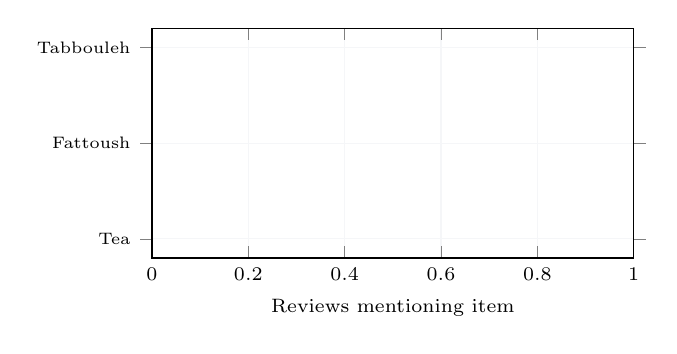
\begin{tikzpicture}\begin{axis}[xbar,width=7.7cm,height=4.5cm,xmin=0,xmax=7,symbolic y coords={MixedGrill,Tea,Fattoush,Tabbouleh,Mansaf},xtick={0,1,2,3,4,5,6},ytick=data,yticklabels={Mixed Grill,Tea,Fattoush,Tabbouleh,Mansaf},y tick label style={font=\fontsize{6.2}{7.2}\selectfont},xticklabel style={font=\scriptsize},grid=major,grid style={LightGray},xlabel={Reviews mentioning item},xlabel style={font=\scriptsize}]\addplot[fill=Teal,draw=Teal] coordinates {(\DiscussedDishThreeMentions,MixedGrill) (\DiscussedDishFiveMentions,Tea) (\DiscussedDishFourMentions,Fattoush) (\DiscussedDishTwoMentions,Tabbouleh) (\DiscussedDishOneMentions,Mansaf)};\end{axis}\end{tikzpicture}\column{0.43\textwidth}\smallcapslabel{Qualified by rating threshold}\par{\fontsize{7.5}{9}\selectfont Mansaf \MansafMentions\ mentions, whole-review avg. \MansafReviewAverage; Tabbouleh \TabboulehMentions, avg. \TabboulehReviewAverage. Fewer than three dishes qualify, so no comparative highest/lowest ranking is shown.}\par\vspace{0.12cm}\smallcapslabel{Negative item evidence}\par{\fontsize{7.5}{9}\selectfont Mixed Grill: \MixedGrillMentions\ mentions, \MixedGrillNegative\ negative; whole-review avg. \MixedGrillReviewAverage; \MixedGrillEvidence\ evidence.}\end{columns}
  \vfill{\color{Gray}\fontsize{6.3}{7.5}\selectfont Review period \EarliestReviewDate-\LatestReviewDate. Whole-review rating is not a guaranteed dish-specific score.}\par\vspace{0.07cm}\goldbutton{a-dishes}{View all 16 dishes/items}
\end{frame}

\chapterdivider{12}{Management Observations}{Customer evidence, internal observations, data needs, experiments and recommendations are different sources.}{Blurring provenance can turn hypotheses into apparent facts.}{Label every claim and approve experiments explicitly.}{m-ch12}{Teal}

\begin{frame}{Separate evidence, observations, experiments and decisions}
  \hypertarget{m-ch12-content}{}\hypertarget{m-observations}{}\sectiontag{Chapter 12 - Management Observations}
  \begin{columns}[T,onlytextwidth]\column{0.48\textwidth}\sourceReview\par\vspace{0.06cm}{\fontsize{7.6}{9.1}\selectfont Drinks/bar has low observable review attention; menu/tablet confusion appears in customer evidence.}\par\vspace{0.13cm}\sourceInternal\par\vspace{0.06cm}{\fontsize{7.6}{9.1}\selectfont Static menu, manual favourites, no recurring offers/bundles, parking visibility and current welcome/guidance are business observations.}\par\vspace{0.13cm}\sourceExperiment\par\vspace{0.06cm}{\fontsize{7.6}{9.1}\selectfont Welcome gesture, weekly feature, bundle, drink feature and richer dish media are tests.}\column{0.48\textwidth}\sourceData\par\vspace{0.06cm}{\fontsize{7.6}{9.1}\selectfont POS orders, revenue, margin, returns and time patterns are required.}\par\vspace{0.13cm}\badge{PaleTeal}{MANAGEMENT ACTION}\par\vspace{0.06cm}{\fontsize{7.6}{9.1}\selectfont Buffet needs dedicated feedback and quality monitoring.}\par\vspace{0.13cm}\badge{PaleGold}{MEASUREMENT PRINCIPLE}\par\vspace{0.06cm}{\fontsize{7.6}{9.1}\selectfont Lifetime rating moves slowly; weekly control should use rolling 30d/90d.}\end{columns}
  \vfill\goldbutton{a-observations}{View provenance register}
\end{frame}

\chapterdivider{13}{Action Plan}{Immediate recovery work is distinct from evidence-dependent menu and operating changes.}{Premature redesign would outrun POS readiness and hide ownership.}{Execute week 1 now; use week 2 for data/hypotheses; test and decide later.}{m-ch13}{Gold}

\begin{frame}{Separate immediate recovery from evidence-dependent change}
  \hypertarget{m-ch13-content}{}\hypertarget{m-actions}{}\sectiontag{Chapter 13 - Action Plan}
  \begin{columns}[T,onlytextwidth]\column{0.48\textwidth}\colorbox{PaleRed}{\parbox[c][4.45cm][t]{0.94\linewidth}{\vspace{0.13cm}{\color{Red}\fontsize{13}{15}\selectfont\bfseries Immediate}\par\vspace{0.10cm}\begin{itemize}\setlength\itemsep{0.07cm}\fontsize{7.8}{9.3}\selectfont\item Assign response owner and log cases\item Reply to open recent reviews\item Check Service/Food cases\item Start rolling KPI dashboard\item Brief staff on menu/buffet/drinks guidance\item Assign competitor/market tasting visits\end{itemize}\vfill\redbutton{a-actions}{Open immediate checklist}}}\column{0.48\textwidth}\colorbox{PaleTeal}{\parbox[c][4.45cm][t]{0.94\linewidth}{\vspace{0.13cm}{\color{Teal}\fontsize{13}{15}\selectfont\bfseries Evidence-dependent}\par\vspace{0.10cm}\begin{itemize}\setlength\itemsep{0.07cm}\fontsize{7.8}{9.3}\selectfont\item Week 2: export/clean POS data\item Define fields and redesign hypotheses\item Define favourite-selection method\item Choose first controlled tests\item Weeks 3-4: test, review, decide\item Repeat market scan and compare evidence\end{itemize}\vfill\tealbutton{a-week2}{Open Week 2 plan}}}\end{columns}
  \vfill\goldbutton{a-market-scan}{View competitor/market assignment}\quad\tealbutton{a-tests}{View test-and-decide plan}
\end{frame}

\chapterdivider{14}{Delegation \& Ownership}{Seven fragmented workstreams can be simplified into four accountable responsibility groups.}{Clear ownership reduces handoffs while preserving manager accountability.}{Delegate deliverables and KPIs; review evidence, blockers and dates weekly.}{m-ch14}{Teal}

\begin{frame}{Four workstreams; the manager keeps accountability}
  \hypertarget{m-ch14-content}{}\hypertarget{m-delegation}{}\sectiontag{Chapter 14 - Delegation \& Ownership}
  \begin{columns}[T,onlytextwidth]\column{0.48\textwidth}\colorbox{PaleGold}{\parbox[c][1.81cm][t]{0.94\linewidth}{\vspace{0.06cm}\textbf{1. Reputation \& Data}\par{\fontsize{7}{8.3}\selectfont Reviews, responses, cases, dashboard and evidence. Owner: Admin/marketing or manager.}}}\par\vspace{0.06cm}\colorbox{PaleTeal}{\parbox[c][1.81cm][t]{0.94\linewidth}{\vspace{0.06cm}\textbf{2. Guest Experience}\par{\fontsize{7}{8.3}\selectfont Welcome, menu guidance, waiting, communication and buffet service. Owner: Service lead.}}}\column{0.48\textwidth}\colorbox{PaleRed}{\parbox[c][1.81cm][t]{0.94\linewidth}{\vspace{0.06cm}\textbf{3. Kitchen \& Buffet Quality}\par{\fontsize{7}{8.3}\selectfont Food cases, dish quality, freshness, consistency and buffet checks. Owner: Kitchen lead.}}}\par\vspace{0.06cm}\colorbox{LightGray}{\parbox[c][1.81cm][t]{0.94\linewidth}{\vspace{0.06cm}\textbf{4. Menu, Bar \& Offers}\par{\fontsize{7}{8.3}\selectfont POS analysis, hypotheses, favourites, offers, drinks and media. Owner: Manager + lead.}}}\end{columns}
  \vfill\implication{Delegate ownership, not accountability. The manager reviews result, evidence, blocker, next action and deadline weekly.}\par\vspace{0.07cm}\goldbutton{a-workstreams}{View responsibilities, KPIs and escalation}
\end{frame}

\chapterdivider{15}{KPI Tracking}{Weekly control needs rolling review, follow-up, operational and experiment indicators.}{The lifetime Google rating moves too slowly to manage weekly execution.}{Use the current 30d baseline and review rolling 30d/90d every week.}{m-ch15}{Gold}

\begin{frame}{Weekly KPI dashboard: four control blocks}
  \hypertarget{m-ch15-content}{}\hypertarget{m-kpi}{}\sectiontag{Chapter 15 - KPI Tracking}
  \begin{columns}[T,onlytextwidth]\column{0.48\textwidth}\colorbox{PaleTeal}{\parbox[c][2.0cm][t]{0.94\linewidth}{\vspace{0.09cm}\smallcapslabel{1. Weekly review KPIs}\par{\fontsize{7.2}{8.6}\selectfont New reviews; new-review average; negative share; low-score cases. \textbf{Baseline:} \RecentThirtyPerWeek/week, \RecentThirtyAverage\ average, \RecentThirtyNegativePct\% negative.}}}\par\vspace{0.10cm}\colorbox{PaleGold}{\parbox[c][2.0cm][t]{0.94\linewidth}{\vspace{0.09cm}\smallcapslabel{2. Follow-up KPIs}\par{\fontsize{7.2}{8.6}\selectfont Owner response rate; low-score response; delay; open cases. \textbf{Baseline:} \OwnerRecentThirtyRate\% recent response.}}}\column{0.48\textwidth}\colorbox{PaleRed}{\parbox[c][2.0cm][t]{0.94\linewidth}{\vspace{0.09cm}\smallcapslabel{3. Operational KPIs}\par{\fontsize{7.2}{8.6}\selectfont Service negatives; Food/Taste negatives; menu complaints; Drinks attention; Buffet sentiment. Show count, percentage and evidence.}}}\par\vspace{0.10cm}\colorbox{LightGray}{\parbox[c][2.0cm][t]{0.94\linewidth}{\vspace{0.09cm}\smallcapslabel{4. Experiment KPIs}\par{\fontsize{7.2}{8.6}\selectfont Offer uptake; bundle uptake; welcome feedback; eligible orders; revenue/margin; POS/order impact. Currently unavailable until tests begin.}}}\end{columns}
  \vfill\colorbox{Navy}{\parbox{0.965\linewidth}{\color{white}\fontsize{7.4}{8.8}\selectfont Lifetime Google rating moves slowly. Use rolling 30d for fast feedback and rolling 90d for stability; review the lifetime score monthly.}}\par\vspace{0.07cm}\goldbutton{a-kpi}{View KPI definitions}
\end{frame}

\chapterdivider{16}{Evidence Appendix}{The management story is traceable to dated registers, charts, anonymous excerpts and public review links.}{Decision-makers can inspect detail without overloading the main narrative.}{Open the relevant appendix, then return to the exact source slide.}{m-ch16}{Teal}

\begin{frame}{Evidence Appendix Roadmap - performance and cases}
  \hypertarget{m-ch16-content}{}\hypertarget{a-index}{}\sectiontag{Chapter 16 - Evidence Appendix}
  \begin{columns}[T,onlytextwidth]\column{0.48\textwidth}{\fontsize{7.2}{8.6}\selectfont\textbf{Appendix A - Latest 30 Days}\par Summary plus all 14 cases, topics, language, response and original links.\par\vspace{0.13cm}\textbf{Appendix B - Previous 30 Days}\par All six comparison cases with the same fields.\par\vspace{0.13cm}\textbf{Appendix C - Bad-Review Register}\par All 30 low-score cases with proposed owner, deadline, check and closure status.\par\vspace{0.13cm}\textbf{Appendix D - Bad-Review Patterns}\par Areas, co-occurrences, recent shift and data gaps.}\column{0.48\textwidth}{\fontsize{7.2}{8.6}\selectfont\textbf{Appendix E - Service}\par All negative Service cases.\par\vspace{0.13cm}\textbf{Appendix F - Food/Taste}\par All negative Food/Taste/quality cases.\par\vspace{0.13cm}\textbf{Appendix G - Bar/Drinks}\par Negative and neutral drink cases.\par\vspace{0.13cm}\textbf{Appendix H - Buffet}\par Negative and neutral buffet cases.}\end{columns}
  \vfill\redbutton{a-bad-register}{Open 30 bad-review cases}\quad\tealbutton{a-latest-register}{Open latest 14 cases}\quad\goldbutton{a-service}{Open Service evidence}
\end{frame}

\begin{frame}{Evidence Appendix Roadmap - operations and action}
  \hypertarget{m-appendix-roadmap-2}{}\sectiontag{Chapter 16 - Evidence Appendix}
  \begin{columns}[T,onlytextwidth]\column{0.48\textwidth}{\fontsize{7.2}{8.6}\selectfont\textbf{Appendix I - Menu/Tablet}\par Complaint and neutral cases.\par\vspace{0.13cm}\textbf{Appendix J - Dishes/Items}\par All 16 items with counts, sentiment, average, evidence, latest date, excerpt and link.\par\vspace{0.13cm}\textbf{Appendix K - Owner Response}\par Period chart, delay and low-score response.\par\vspace{0.13cm}\textbf{Appendix L - Provenance}\par Corrected evidence/observation/action labels.}\column{0.48\textwidth}{\fontsize{7.2}{8.6}\selectfont\textbf{Appendix M - Action System}\par Immediate checklist; Week 2 data setup; tests; market scan; four workstreams; response process; POS matrix.\par\vspace{0.13cm}\textbf{Appendix N - KPI Control}\par Definitions, cadence, owner and baseline.\par\vspace{0.20cm}\colorbox{PaleGold}{\parbox{0.92\linewidth}{\fontsize{7}{8.4}\selectfont Gold = evidence/action detail. Teal = case/data detail. Red = bad-review registers. Every appendix page has a visible Back button.}}}\end{columns}
  \vfill\goldbutton{a-dishes}{Open all dishes}\quad\tealbutton{a-actions}{Open action checklist}\quad\backbutton{m-roadmap}{Back to Presentation Roadmap}
\end{frame}

\input{presentation_appendix.tex}

\end{document}
